\documentclass[11pt]{article}
\usepackage[top=2.1cm,bottom=2cm,left=2cm,right= 2cm]{geometry}
%\geometry{landscape}                % Activate for for rotated page geometry
\usepackage[parfill]{parskip}    % Activate to begin paragraphs with an empty line rather than an indent
\usepackage{graphicx}
\usepackage{amssymb}
\usepackage{epstopdf}
\usepackage{amsmath}
\usepackage{multirow}
\usepackage{hyperref}
\usepackage{changepage}
\usepackage{lscape}
\usepackage{ulem}
\usepackage{multicol}
\usepackage{dashrule}
\usepackage[usenames,dvipsnames]{color}
\usepackage{enumerate}
\newcommand{\urlwofont}[1]{\urlstyle{same}\url{#1}}
\newcommand{\degree}{\ensuremath{^\circ}}
\newcommand{\hl}[1]{\textbf{\underline{#1}}}



\DeclareGraphicsRule{.tif}{png}{.png}{`convert #1 `dirname #1`/`basename #1 .tif`.png}

\newenvironment{choices}{
\begin{enumerate}[(a)]
}{\end{enumerate}}

%\newcommand{\soln}[1]{\textcolor{MidnightBlue}{\textit{#1}}}	% delete #1 to get rid of solutions for handouts
\newcommand{\soln}[1]{ \vspace{1.35cm} }

%\newcommand{\solnMult}[1]{\textbf{\textcolor{MidnightBlue}{\textit{#1}}}}	% uncomment for solutions
\newcommand{\solnMult}[1]{ #1 }	% uncomment for handouts

%\newcommand{\pts}[1]{ \textbf{{\footnotesize \textcolor{black}{(#1)}}} }	% uncomment for handouts
\newcommand{\pts}[1]{ \textbf{{\footnotesize \textcolor{blue}{(#1)}}} }	% uncomment for handouts

\newcommand{\note}[1]{ \textbf{\textcolor{red}{[#1]}} }	% uncomment for handouts

\begin{document}


\enlargethispage{\baselineskip}

Spring 2021 \hfill Jingchen (Monika) Hu\\

\begin{center}
{\huge MATH 241 Homework 1 Questions}	\\
Due: Sunday 2/28 11:59pm to Moodle
\end{center}
\vspace{0.5cm}


%%%%%%%%%%%%%%%%%%%%%%%%%%%%%%%%%%%%%%%%%%%%%%
\begin{itemize}

    \item
    Chapter 1 Problem 3
    
    Twenty workers are to be assigned to 20 different jobs, one to each job. How many different assignments are possible?
    
    \item
    Chapter 1 Problem 5
    
    For years, telephone area codes in the United States and Canada considered a sequence of three digits. The first digit was an integer between 2 and 9, the second digit was either 0 or 1, and the third digit was any integer from 1 to 9. How many area codes were possible? How many area codes starting with a 4 were possible?
    
    \item
    Chapter 1 Problem  7
    
    \begin{enumerate}[(a)]
    \item In how many ways can 3 boys and 3 girls sit in a row?
    \item In how many ways can 3 boys and 3 girls sit in a row if the boys and the girls are each to sit together?
    \item In how many ways if only the boys must sit together?
    \item In how many ways if no two people of the same sex are allowed to sit together?
    \end{enumerate}
    
    \item
    Chapter 1 Problem  8
    
    How many different letter arrangements can be made from letters
    
    \begin{enumerate}[(a)]
    \item Fluke?
    \item Propose?
    \item Mississippi?
    \item Arrange?
    \end{enumerate}

    \item
    Chapter 1 Problem  13
    
    Consider a group of 20 people. If everyone shakes hands with everyone else, how many handshakes take place?

    \item
    Chapter 1 Problem  15
    
    A dance class consists of 22 students of which 10 are women and 12 are men. If 5 men and 5 women are to be chosen and then paired off, how many results are possible?

    \item
    Chapter 1 Problem  19
    
    From a group of 8 women and 6 men, a committee consisting of 3 men and 3 women is to be formed. How many different committees are possible if
    
    \begin{enumerate}[(a)]
    \item 2 of the men refuse to serve together?
    \item 2 of the women refuse to serve together?
    \item 1 man and 1 woman refuse to serve together?
    \end{enumerate}

    \item
    Chapter 1 Problem  21
    
    Consider the grid of points shown here. Suppose that, starting at the point labeled $A$, you can go one step up or one step to the right at each move. This procedure is continued until the point labeled $B$ is reached. How many different paths from $A$ to $B$ are possible? [Hint: Note that to reach $B$ from $A$, you must take 4 steps to the right and 3 steps upward.]
    
   \begin{center}
   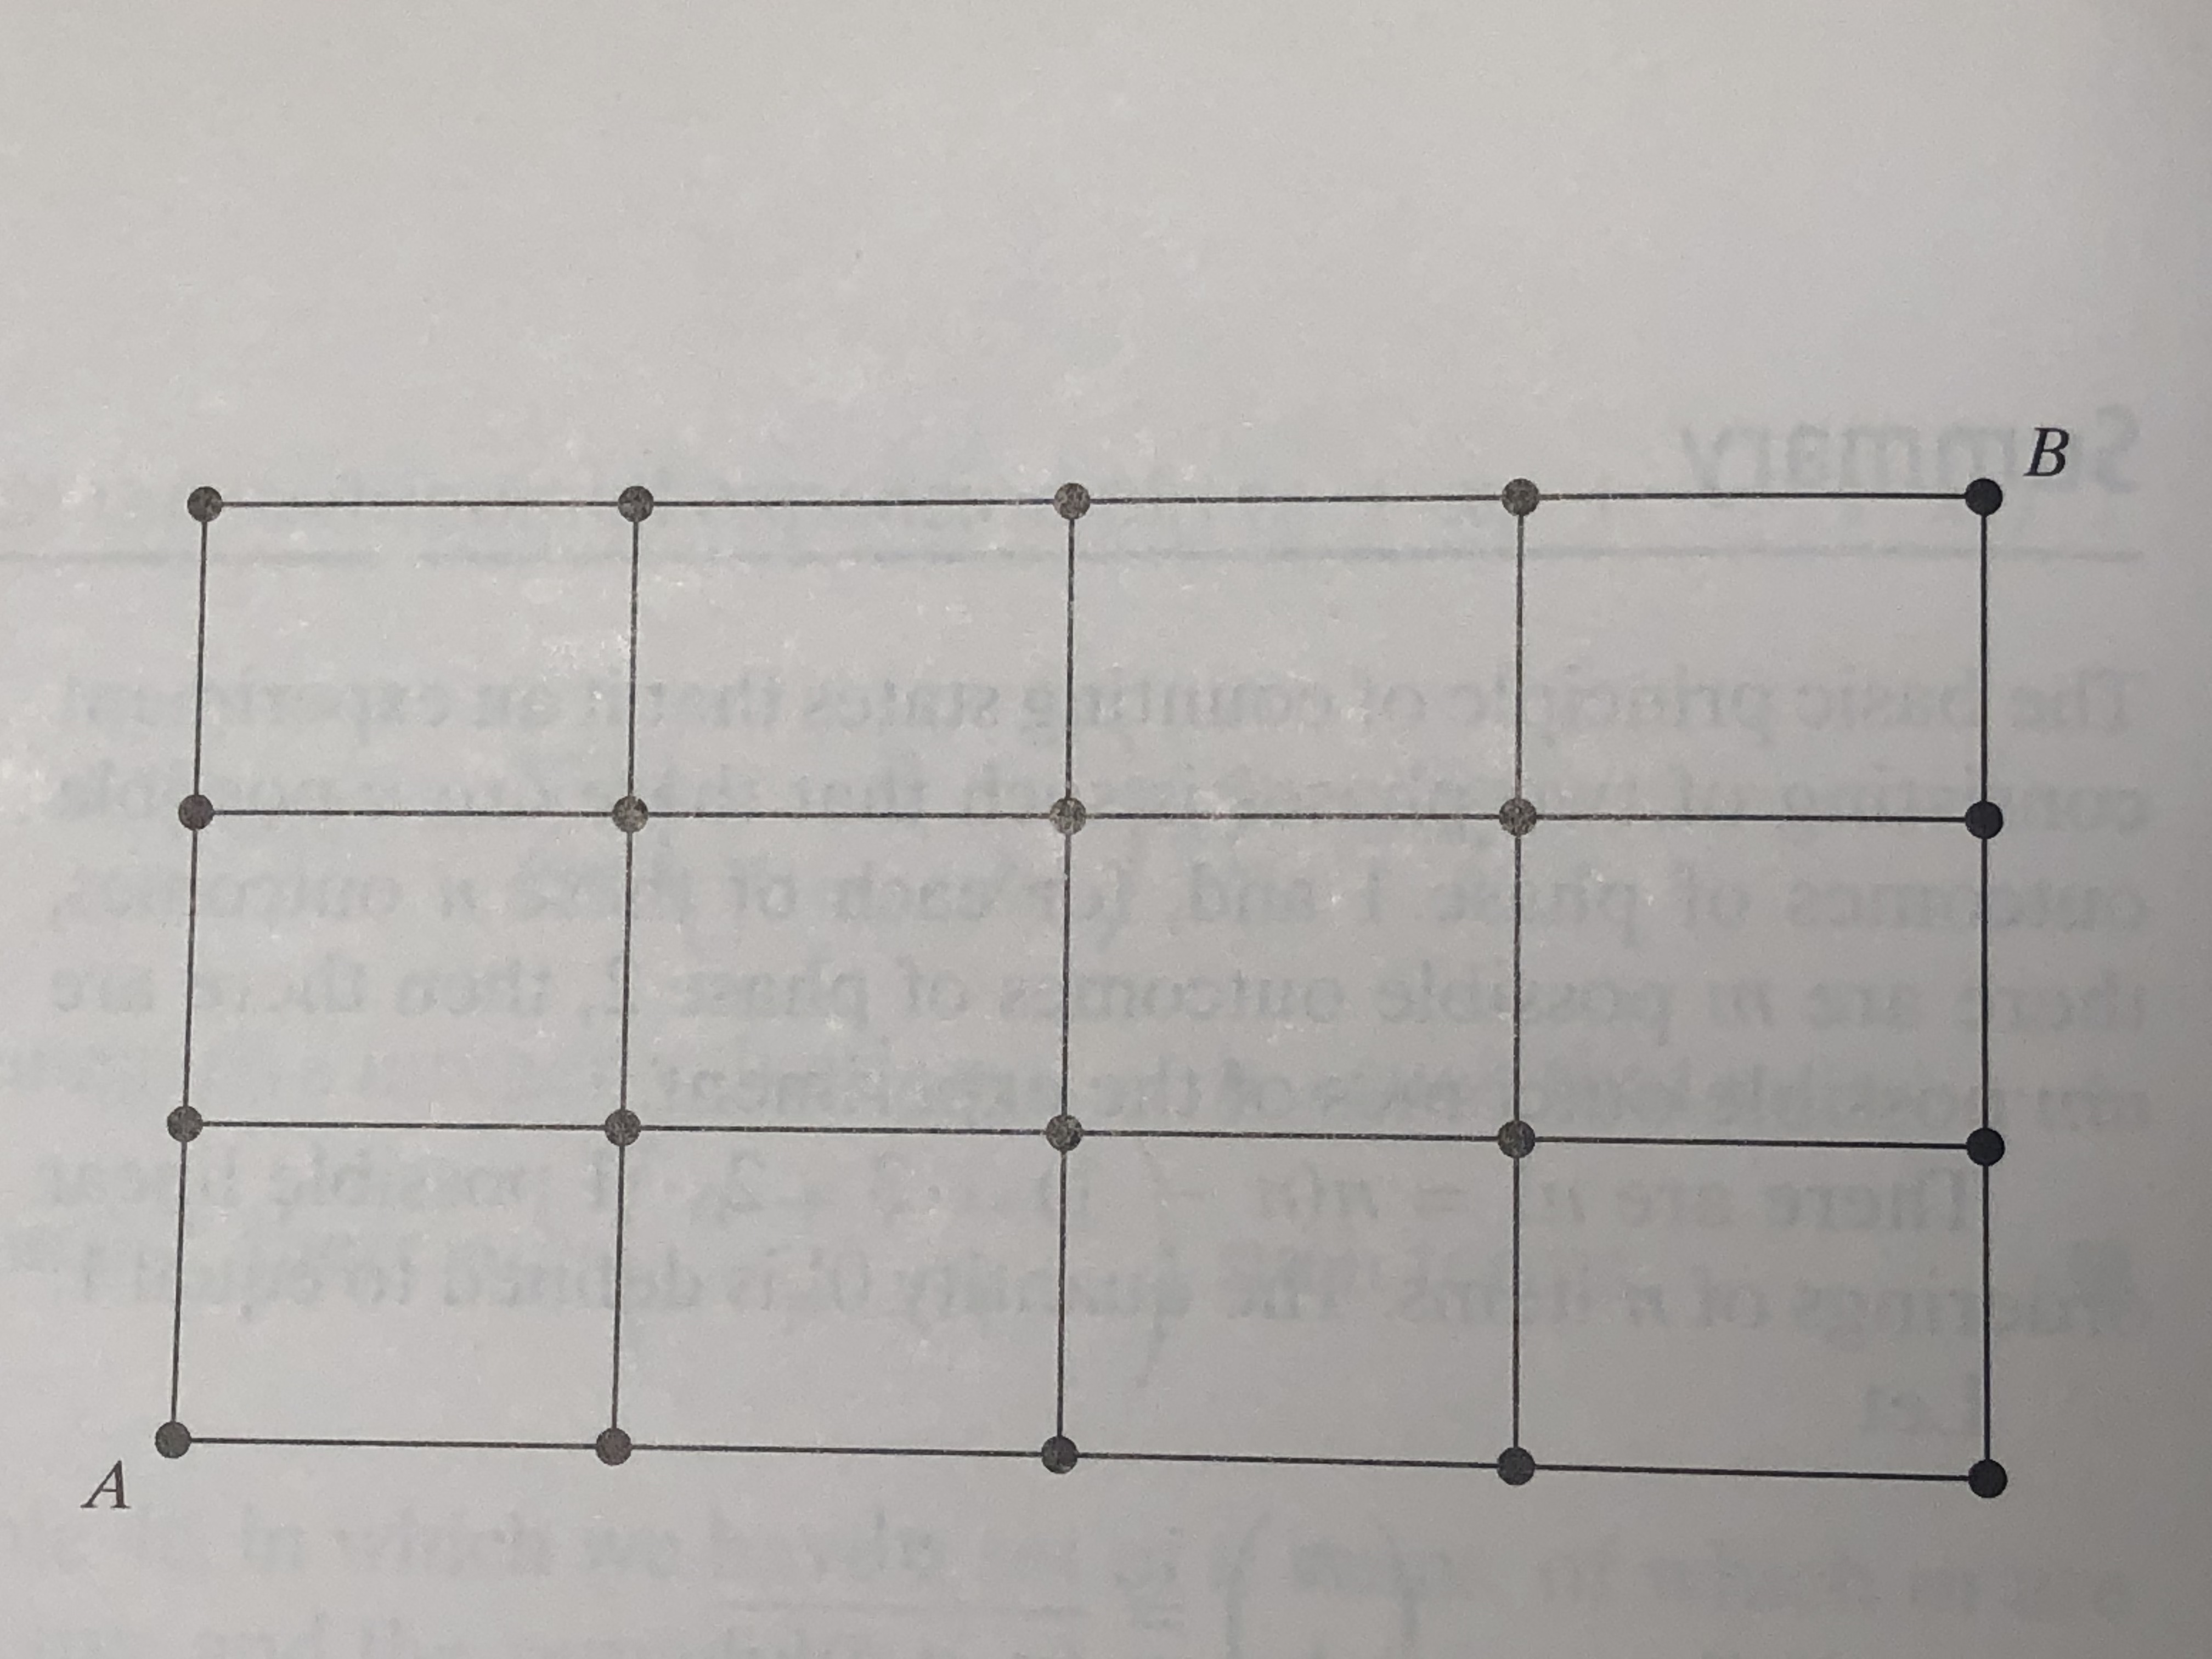
\includegraphics[scale=0.05]{Q21}
   \end{center}
   
    \item
    Chapter 1 Problem  22
    
    In Problem 21, how many different paths are there from $A$ to $B$ that go through the point circled in the following lattice?
    
    \begin{center}
   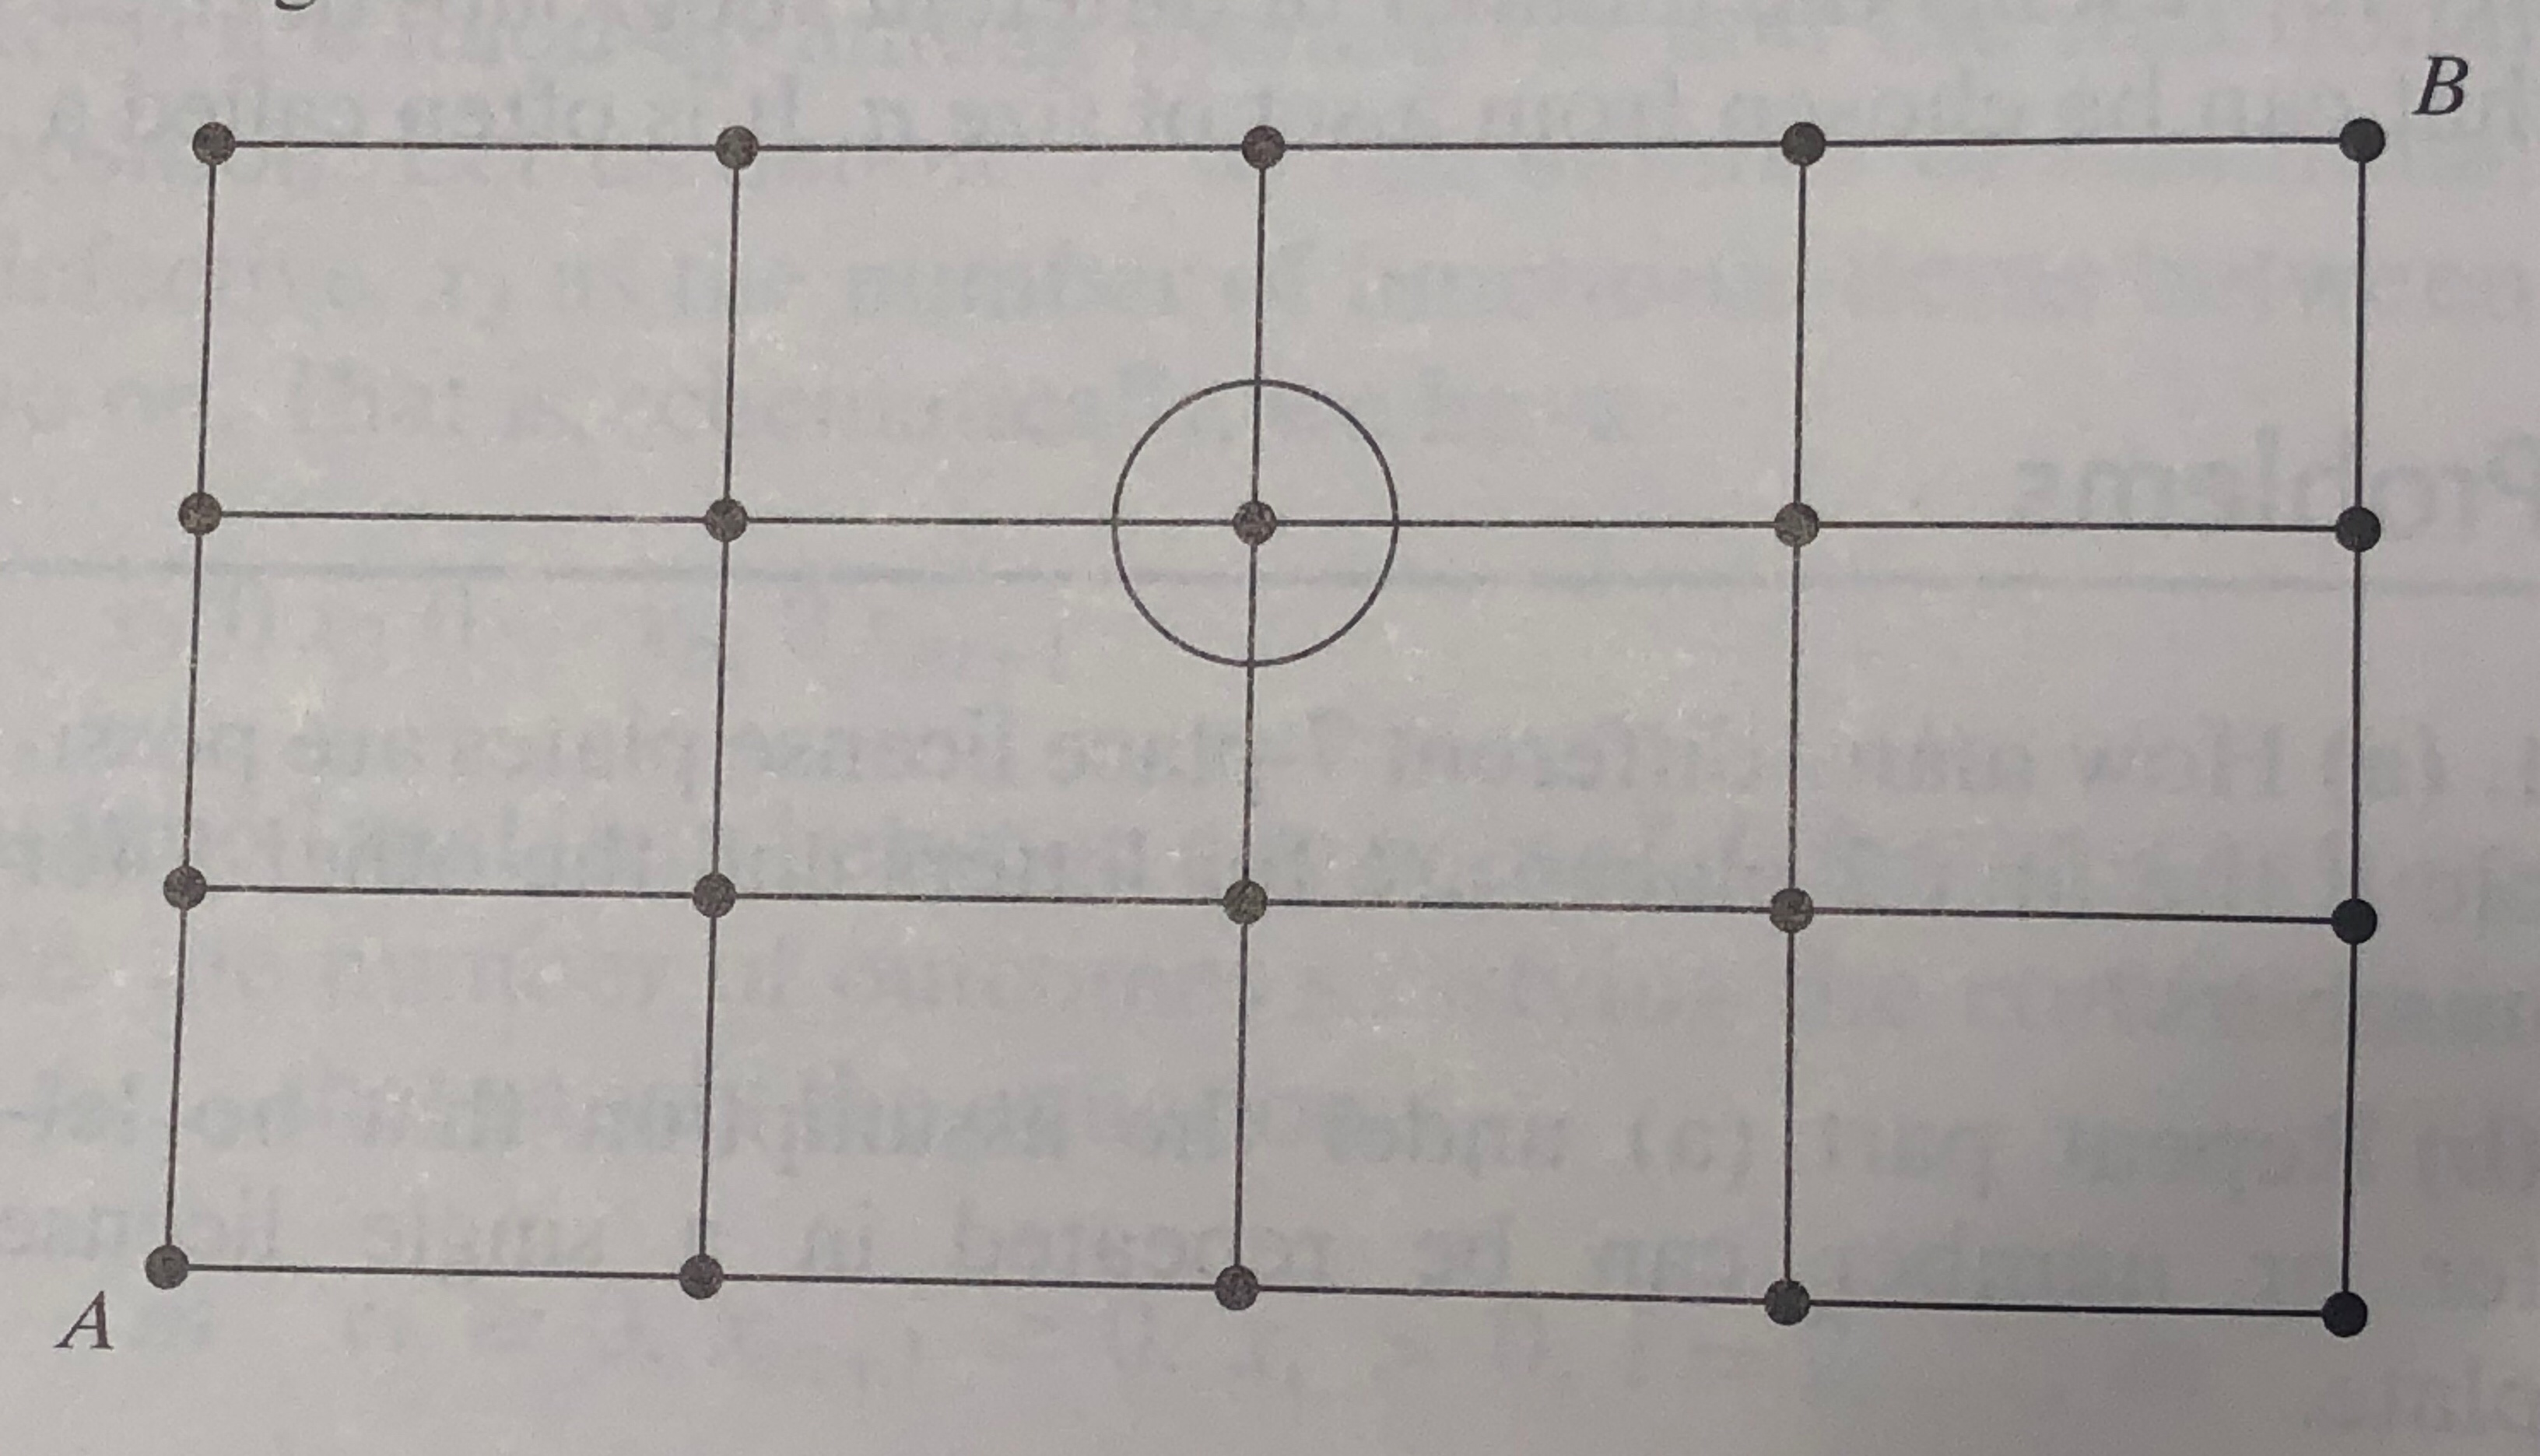
\includegraphics[scale=0.07]{Q22}
   \end{center}

    \item
    Chapter 1 Problem  24

    Expand $(3x^2 + y)^5$.
    
    \item
    Chapter 1 Problem  27
    
    If 12 people are to be divided into 3 committees of respective size 3, 4, and 5, how many divisions are possible?

    \item
    Chapter 1 Theoretical exercise 2
    
    Two experiments are to be performed. The first can result in any one of $m$ possible outcomes. If the first experiment results in outcome $i$, then the second experiment can result in any of $n_i$ possible outcomes, $i = 1, 2, \cdots, m$. What is the number of possible outcomes of the two experiments?

    \item
    Chapter 1 Theoretical exercise 8

    Prove that
    
    $$
    {n+m \choose r} = {n \choose 0}{m \choose r} + {n \choose 1}{m \choose r-1} + \cdots + {n \choose r}{m \choose 0}
    $$
    
    [Hint: Consider a group of $n$ men and $m$ women. How many groups of size $r$ are possible?]
    
    \item
    Chapter 1 Theoretical exercise 9
    
    Use Theoretical Exercise 8 to prove that
    
    $$
    {2n \choose n} = \sum_{k=0}^n {n \choose k}^2
    $$
    
    \item
    Chapter 1 Theoretical exercise 13
    
    Show that, for $n > 0$,
    
    $$
    \sum_{i=0}^n (-1)^i {n \choose i} = 0
    $$
    
    [Hint: Use the binomial theorem.]


\end{itemize}

\vspace{12pt}

\underline{Optional: if you feel like more practice}\\
These will not be graded, but you are welcome to discuss these with me during the office hour. 

\begin{itemize}

%%%%%%%%%%%%%%%%%%%%%%%%%%%%%%%%%%%%%%%%%%%%%%

\item Textbook  Chapter 1 Problems: 1, 2, 4, 6, 9, 10, 11, 12, 16, 17, 18, 20, 23, 30
\item Textbook  Chapter 1 Theoretical exercise: 10, 11



\end{itemize}



\end{document} 